%----------------------------------------------------------------------
\chapter[Astronomy introduction]{Astronomy introduction}
%----------------------------------------------------------------------
 
We usually refer to celestial mechanics, astrodynamics, orbital dynamics, attitude dynamics or astronomy as the same thing. However it is important to make clear that these concepts differ from each other and we should properly understand what we refer to when talking about each one. Let us start this chapter by defining them in detail:

\vspace{0.25cm}
\begin{Definition*}{}
	\textbf{Celestial mechanics} is the scientific study of celestial body dynamics.
\end{Definition*}
\vspace{0.25cm}

\vspace{0.25cm}
\begin{Definition*}{}
	\textbf{Orbital dynamics} is the scientific study of the motion of small orbiting bodies.
\end{Definition*}
\vspace{0.25cm}

\vspace{0.25cm}
\begin{Definition*}{}
	\textbf{Attitude dynamics} is the scientific study of the relative position and orientation of bodies in space.
\end{Definition*}
\vspace{0.25cm}

\vspace{0.25cm}
\begin{Definition*}{}
	\textbf{Astronomy} is  the scientific study of matter and phenomena in the universe, especially in outer space, including the positions, dimensions, distribution, motion, composition, energy, and evolution of celestial objects.
\end{Definition*}
\vspace{0.25cm}

\begin{Definition*}{}
	\textbf{Astrodynamics} is the branch of astronomy that studies the motion of celestial and man-made bodies in space subjected to both natural and artificial perturbations.
\end{Definition*}
\vspace{0.25cm}

\section{The Solar System models}

When first human beings started to look at the stars, they tried to explain 

\begin{figure}[h]
	\centering
	
\includegraphics[scale=0.75]{figs/sky_path.png}
	\caption{Apparent path of a celestial body}
\end{figure}


\newpage
\section{The Solar System and its main bodies}
In this section, the Solar System 

% ----------- MERCURY PLANET INFORMATION ----------
\newpage
\subsection{Mercury}
\begin{wrapfigure}{r}{0.55\textwidth}
	\begin{center}
		\includegraphics[width=0.5\textwidth]{figs/spacecraft/mariner10.png}
	\end{center}
	\caption{Mariner 10 spacecraft drawing}
\end{wrapfigure}
Mercury is the most inner planet that orbits the Sun, which makes difficult to observe from Earth. It completes an orbit around the Sun in approximately 88 Earth days. This is the main reason behind its name: the fleet-flooted messenger of the gods. In addition, the chemical element mercury is also a quick-flowing silvery liquid.\\

When the Mariner 10 spacecraft orbited the planet, it took some pictures of the surface. They revealed a heavily cratered planet similar to our Moon's surface. The spacecraft also discovered a magnetic field $10^{-4}$ times the Earth one. However, due to its small size, the planet has lost all its internal energy and thus it is no longer geologically active. After Mariner mission, the MESSENGER spacecraft revealed the biggest ringed area: the Caloris Basin, which has a 1300[km] diameter.\\

Mercury does not have an atmosphere since the solar wind is so strong in this region. The planet is quite dense and mission data indicates that its core should be composed by a large metallic core, which is supposed to occupy around 70\% of planet's radius. As a brief resume, Mercury is a metal planet with a tiny rock mantle.

\begin{figure}[h]
	\centering
	\includegraphics[scale=0.75]{figs/bodies/mercury.png}
	\caption{Mercury data}
\end{figure}

% ----------- VENUS PLANET INFORMATION ----------
\subsection{Venus}
\begin{figure}[h]
	\centering
	\includegraphics[scale=0.75]{figs/bodies/venus.png}
	\caption{Venus data}
\end{figure}
